Sei \(f\colon\mathcal{M}\looparrowright\mathcal{N}\) eine Immersion. Dann faktorisiert \(\dx f\) durch die kanonische Abbildung \(f^*T\mathcal{N}\to T\mathcal{N}\) und es existiert ein kommutatives Diagramm
\begin{center}
    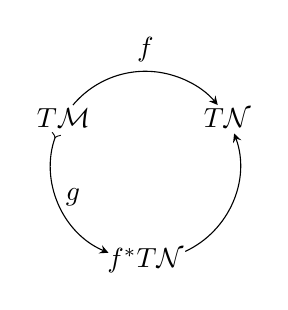
\begin{tikzpicture}[scale = 0.8]
        \draw
            (30:1.5) node (A) {\(T\mathcal{N}\)}
            (150:1.5) node (B) {\(T\mathcal{M}\)}
            (270:1.5) node (C) {\(f^*T\mathcal{N}\)}
            ;
            \draw [-stealth] (140:1.5) arc (140:40:1.5) node [pos = 0.5, above] {\(\dx f\)};
            \draw [>-stealth] (160:1.5) arc (160:247:1.5) node [pos = 0.45, right] {\(g\)};
            \draw [-stealth] (295:1.5) arc (295:380:1.5);
    \end{tikzpicture}
\end{center}
sodass sich das Normalenb\"undel von \(f\) als \(\nu(f):=f^*T\mathcal{N}/g(T\mathcal{M})\) definieren l\"asst. Ist \(f\) eine Einbettung, entspricht dies gerade dem bekannten Normalenb\"undel. Analog zu der Schnittzahl zweier transversaler Mannigfaltigkeiten kann die Selbstschnittzahl einer Immersion \(f\colon\mathcal{M}^k\looparrowright\mathcal{N}^{2k}\) definiert werden. Es kann zun\"achst angenommen werden, dass \(f\) sich selbst transversal schneide und lediglich endlich viele Doppelpunkte \(f(p)=f(q)\) besitzt. Definiere \(\epsilon_p\) als \(1\), wenn die zusammengesetzte Orientierung von 
\[T_p\mathcal{N}=\dx_pf\left(T_p\mathbb{S}^k\right)\oplus\dx_qf\left(T_q\mathbb{S}^k\right)\]
der gew\"ahlten Orientierung von \(\mathcal{N}\) entspricht und \(-1\) sonst. Ist \(k\) gerade ist, sei die Selbstschnittzahl
\[I_f\mathop{:=\sum\epsilon_p}_{f(p)=f(q)}\,,\]
ist \(k\) ungerade sei sie eben jene Summe modulo zwei. Besonders wichtig ist diese Zahl in der Verwendung des starken Einbettungssatzes von Whitney, also auch in Whitneys Trick. Siehe Abbildung \ref{fig:whitney_trick}.

\begin{proposition}[Whitneys Trick]\label{prop:whit_trick}
    Sei \(k\geq3\), \(\mathcal{N}^{2k}\) einfach zu\-sam\-men\-h\"an\-gend und \(f\colon\mathcal{M}^k\looparrowright\mathcal{N}\) eine Immersion. \"Ubersteigt die Anzahl der Doppelpunkte von \(f\) die Zahl \(\abs{I_f}\), oder ist \(>0\) f\"ur ungerade \(k\), existiert eine regul\"ar homotope Immersion \(g\), die zwei Doppelpunkte weniger besitzt.
\end{proposition}
\begin{proof}
    Siehe \cite{whitney1944intersect} Satz 4.
\end{proof}

\begin{figure}
    \centering
    \begin{tikzpicture}
        \begin{scope}[xshift = -3cm]
            \draw 
                (2, 0) arc (10:170:2 and 1) 
                    node (A) [pos = 0.2] {\tiny\textbullet}
                    node (B) [pos = 0.8] {\tiny\textbullet}
                    node (C) [pos = 0.45] {}
                (2, 1) arc (-10:-170:2 and 1)
                    node (D) [pos = 0.55] {}
                (C.center) edge [densely dotted, -stealth] ++(0, -1.2)
                (D.center) edge [densely dotted, -stealth] ++(0, 1.2)
                ;
            \draw 
                (A) node [above] {\tiny\(q\)} node [below] {\tiny\(1\)}
                (B) node [above] {\tiny\(p\)} node [below] {\tiny\(-1\)}
            ;

            \fill [pattern = north west lines] 
                (A) arc (42:138:2 and 1) arc (-138:-42: 2 and 1) -- cycle;
        \end{scope}
        \draw (-0.75, 0.5) edge [-stealth] (0.75, 0.5);
        \begin{scope}[xshift = 3cm]
            \draw 
                (2, 0) arc (10:170:2 and 0.5) 
                    node (E) [pos = 0.45] {}
                (2, 1) arc (-10:-170:2 and 0.5)
                    node (F) [pos = 0.55] {}
                (E.center) edge [densely dotted, -stealth] ++(0, -0.75)
                (F.center) edge [densely dotted, -stealth] ++(0, 0.75)
                ;
        \end{scope}
    \end{tikzpicture}
    \caption{Die Idee von Whitneys Trick zur Eliminierung der Doppelpunkte \(p\) und \(q\) einer Immersion \(f\colon\mathbb{S}^1\looparrowright\mathcal{N}\). Der einfache Zusammenhang von \(\mathcal{N}\) garantiert, dass der schraffierte Bereich kontrahierbar ist.}\label{fig:whitney_trick}
\end{figure}

\begin{corollary}\label{cor:imm_reg_hom}
    Sei \(k\geq3\) ungerade, \(\mathcal{N}^{2k}\) einfach zusammenh\"angend und \(f\colon\mathcal{M}^k\looparrowright\mathcal{N}^{2k}\) eine Immersion. Die Selbstschnittzahl von \(f\) ist genau dann null, wenn \(f\) regul\"ar homotop zu einer Einbettung ist.
\end{corollary}

\begin{proposition}\label{prop:imm_inter_zero}
    Es existiert eine Immersion \(h\colon\mathbb{S}^k\looparrowright\mathbb{R}^{2k}\) mit Selbstschnittzahl eins.
\end{proposition}
\begin{proof}
    Siehe \cite{whitney1944intersect} Satz 3.
\end{proof}

\begin{figure}[!h]
    \centering
    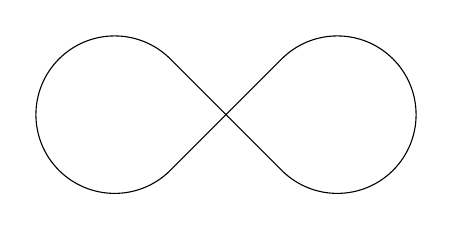
\begin{tikzpicture}
        \draw (-0.707, 0.707) arc (45:315:1) -- (0.707, 0.707) arc (135:-135:1) -- cycle;
    \end{tikzpicture}
    \caption{Eine Immersion \(f\colon\mathbb{S}^1\looparrowright\mathbb{R}^2\) mit Selbstschnittzahl eins.}\label{fig:double_imm}
\end{figure}
